\documentclass{beamer}

\usepackage{tikz}
\usepackage{array}
\usepackage{bbold}
\usepackage{graphicx}
\usepackage[T1]{fontenc}
\usepackage[utf8]{inputenc}

\usetheme{Copenhagen}

\title{CR11 --- Mathematical methods for image synthesis}
\author{Simon Mauras}
\institute{ENS de Lyon}
\date{December 20\textsuperscript{th} 2017}
\setbeamertemplate{footline}[frame number]
\setbeamertemplate{navigation symbols}{}

\begin{document}

\begin{frame}
  \titlepage
\end{frame}

\begin{frame}
  \tableofcontents
\end{frame}

\section{Stable Region Correspondences}

\subsection{Motivations}

\begin{frame}
  \begin{block}{Stable Region Correspondences Between Non-Isometric Shapes}
    V. Ganapathi-Subramanian, B.Thibert, M. Ovsjanikov, L. Guibas
    
    \medskip\textit{Computer Graphics Forum}. Vol. 35. No. 5. 2016.
  \end{block}
  
  \bigskip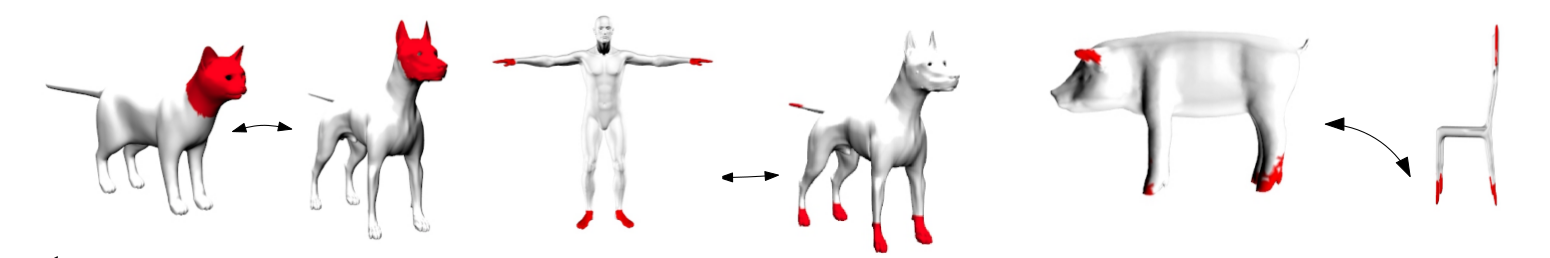
\includegraphics[width=\textwidth]{article/intro.png}
\end{frame}

\subsection{Affinity Matrix}

\begin{frame}
  We are given two shapes as triangulated meshes.
  
  \medskip Vertex sets $S^{(1)} = \{p_1, \dots, p_{d_1}\}$ and $S^{(2)} = \{q_1, \dots, q_{d_2}\}$.
  
  \medskip Feature functions $f^{(1)}$ and $f^{(2)}$ (\textit{e.g.} Gaussian curvature).
  \[f^{(1)} : S^{(1)} \mapsto \mathbb R \quad\text{and}\quad f^{(2)} : S^{(2)} \mapsto \mathbb R\]
  
  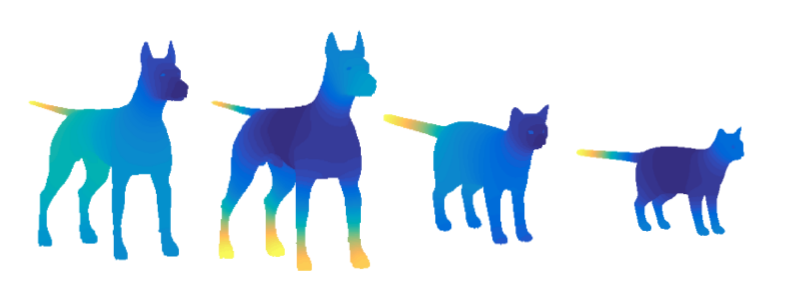
\includegraphics[width=\textwidth]{article/features.png}
  
  Even if values are different, the rank of a value is useful!
\end{frame}

\begin{frame}
  \medskip We define to permutations $r^{(1)}$ and $r^{(2)}$ of $\mathfrak S_n$:
  \[r^{(1)}_i = j \;\text{ if }f^{(1)}(p_j)\text{ is the }i^{th}\text{ value in sorted order.}\]
  \[r^{(2)}_i = j \;\text{ if }f^{(2)}(q_j)\text{ is the }i^{th}\text{ value in sorted order.}\]
  
  \medskip Let $K$ be an integer that divides $d_1$ and $d_2$. For $1 \leq k \leq K$:
  \[C_k^{(1)} = \left\{r^{(1)}_i \;\middle|\; (k-1)\frac{d_1}{K} \lneq i \leq k\frac{d_1}{K} \right\}\]
  \[C_k^{(2)} = \left\{r^{(2)}_i \;\middle|\; (k-1)\frac{d_2}{K} \lneq i \leq k\frac{d_2}{K} \right\}\]
\end{frame}

\begin{frame}
Now we can define the affinity matrix!
\[W = \sum_{k=1}^K \mathbb 1_{C^{(2)}_k} \cdot \mathbb 1_{C^{(1)}_k}^T = \underbrace{\left(\begin{array}{ccc|ccc|ccc}
1 & \dots & 1 & && & && \\
\vdots & & \vdots & &(0)& & &(0)& \\
1 & \dots & 1 & && & && \\\hline
&& & 1 & \dots & 1 & &&\\
&(0)& & \vdots & & \vdots & &(0)&\\
&& & 1 & \dots & 1 & &&\\\hline
&& & && & 1 & \dots & 1\\
&(0)& & &(0)& & \vdots && \vdots\\
&& & && & 1 & \dots & 1\\
\end{array}\right)}_{\displaystyle r^{(1)}_1 \; r^{(1)}_2 \hspace{4cm} r^{(1)}_{d_1}}\left\}\begin{array}{c}r^{(2)}_1\\r^{(2)}_2\\\\\\\\\\\\\\\\r^{(2)}_{d_2}\end{array}\right.\]
Coefficient $i,j$ is $1$ if $f^{(1)}(p_j)$ and $f^{(2)}(q_i)$ have similar ranks...
\end{frame}

\begin{frame}
  Now we consider $N$ different features!
  \par$\rightarrow$ The affinity matrix is the sum of each matrix.
  \par\bigskip
  We need to "normalize" the matrix
  \par$\rightarrow$ Multiply each coefficient by $K/(Nd_1d_2)$.
  \par\bigskip Remark that $(1\;\dots\;1)^T$ is an eigenvector of $W^TW$.
  $\rightarrow W \cdot (1\;\dots\;1)^T = (1/d_1)(1\;\dots\;1)^T$
  $\rightarrow W^T \cdot (1\;\dots\;1)^T = (1/d_2)(1\;\dots\;1)^T$
\end{frame}

\subsection{Stable pairs}

\begin{frame}
  Let $||M||$ be the sum of the absolute value of all coefficients of $M$.
  \par\bigskip
  Let $M_{I,J}$ be the submatrix of $M$ on lines $I$ and columns $J$.
  \par\bigskip
  We are now ready to define a stable pair of size $(n,m)$.
  \par\bigskip
  Subset $\Omega^{(1)} \times \Omega^{(2)} \subseteq S^{(1)} \times S^{(2)}$ with $|\Omega^{(1)}| = n$ and $|\Omega^{(2)}| = m$,
  \\\quad such that $||W_{\Omega^{(2)}, \Omega^{(1)}}||$ is maximal.
\end{frame}

\begin{frame}
  \centering
  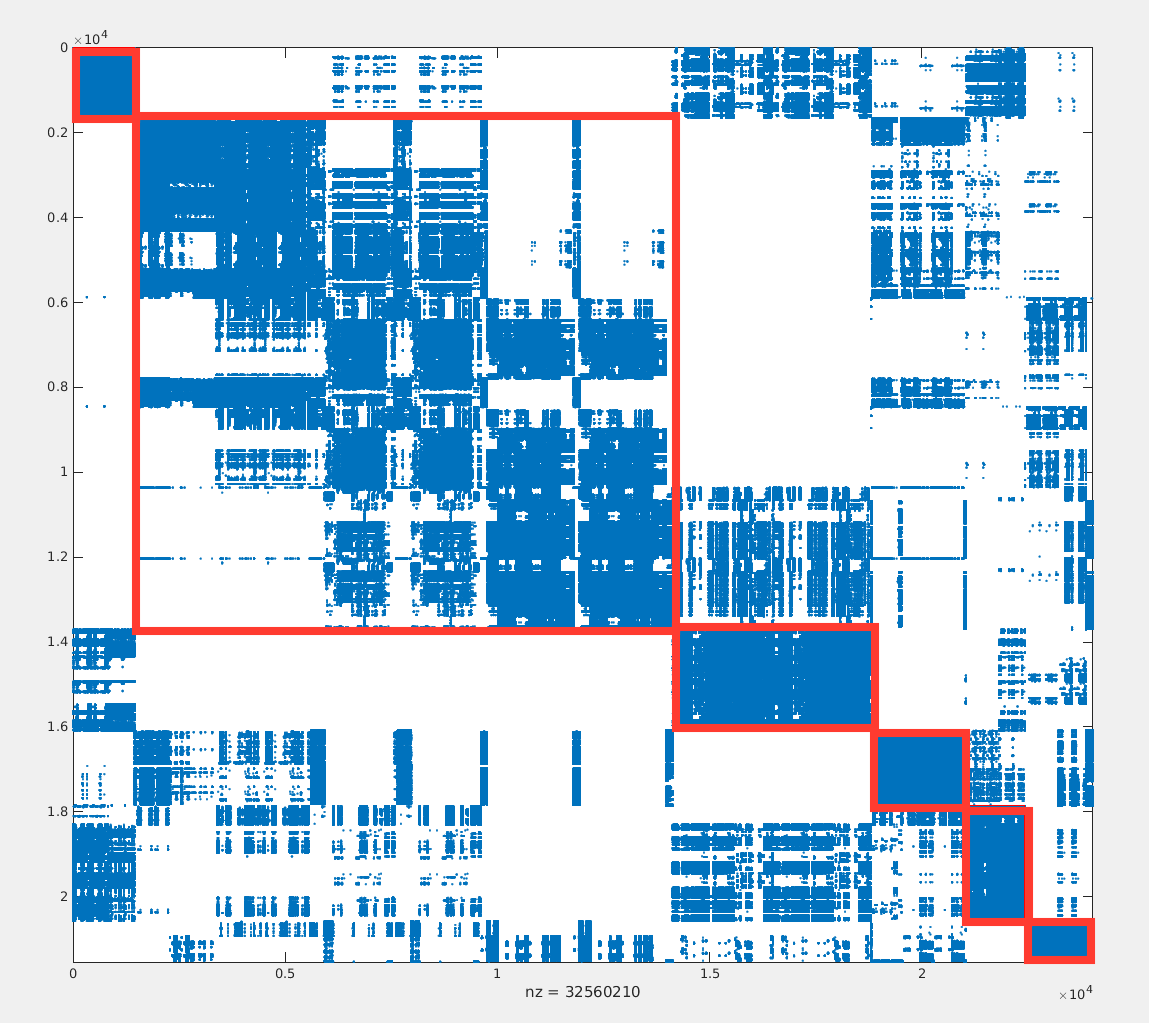
\includegraphics[width=.8\textwidth]{article/matrix.png}
\end{frame}

\begin{frame}
  Several algorithms are given to efficiently compute stable pairs.
  \par\bigskip
  The procedure is stable when adding noise (random i.i.d. features)
  \par\bigskip
  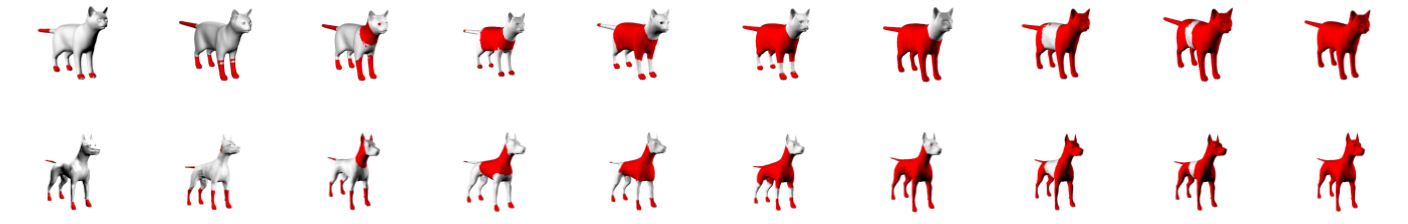
\includegraphics[width=\textwidth]{article/result.png}
  
\end{frame}

\section{Poisson Image Editing}

\subsection{Goal}

\begin{frame}
  \begin{center}
    \begin{tabular}{m{1.6cm}m{.6cm}m{1.6cm}m{.6cm}m{4.7cm}}
      $\overbrace{\hspace{1.6cm}}^{\Omega}$ &&
      $\overbrace{\hspace{1.6cm}}^u$ &&
      $\overbrace{\hspace{4.7cm}}^v$ \\
      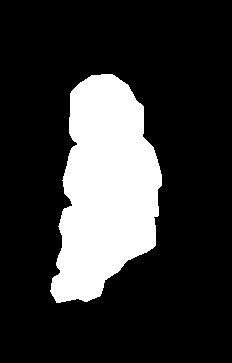
\includegraphics[scale=.2]{results_poisson/foreground-mask.png}
      & {\Huge$\times$} &
      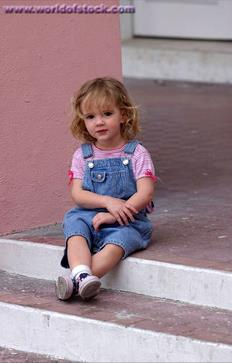
\includegraphics[scale=.2]{results_poisson/foreground.png}
      & {\Huge$+$} &
      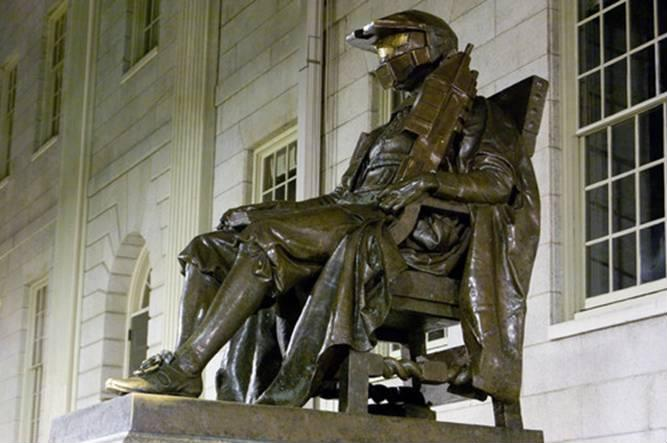
\includegraphics[scale=.2]{results_poisson/background.png}
    \end{tabular}
    \par\medskip
    \begin{tabular}{m{.6cm}m{4.7cm}}
      {\Huge=} &
      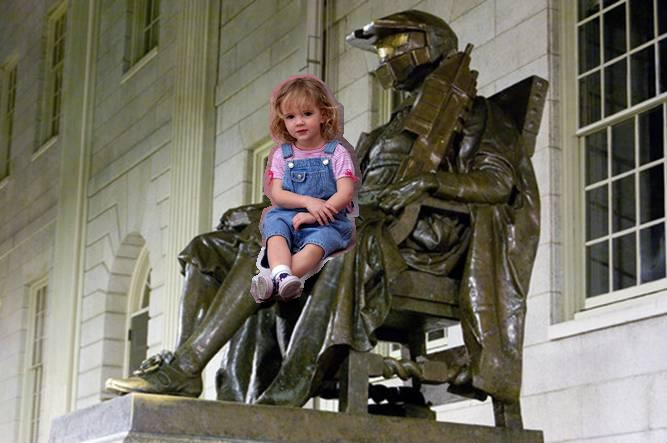
\includegraphics[scale=.2]{results_poisson/naive.png}
    \end{tabular}
  \end{center}
\end{frame}

\subsection{Poisson equation}

\begin{frame}
  Idea : "Shift" the colors, but try keep the shapes.
  
  \medskip Let $\tilde u$ such that $\tilde u = v$ on $\partial\Omega$
  
  \medskip Minimize $\mathcal L(\tilde u) = \int_\Omega |\nabla(\tilde u - u)|^2$
  
  \medskip We deduce a Poisson equation $\nabla^2 \tilde u = 0$ in $\Omega$
  
  \medskip We discretize this equation, with a discrete laplacian operator.
  
  \medskip It's a sparse linear system, we use the conjugate gradiant method.
\end{frame}

\subsection{Results}

\begin{frame}
  \begin{center}
    ~\\
    \includegraphics<1>[width=\textwidth]{results_poisson/background.png}
    \includegraphics<2>[width=\textwidth]{results_poisson/1.png}
    \includegraphics<3>[width=\textwidth]{results_poisson/10.png}
    \includegraphics<4>[width=\textwidth]{results_poisson/100.png}
    \includegraphics<5>[width=\textwidth]{results_poisson/1000.png}
    \includegraphics<6>[width=\textwidth]{results_poisson/10000.png}
    
    \only<1>{Initial image}
    \only<2>{After 1 iteration}
    \only<3>{After 10 iteration}
    \only<4>{After 100 iteration}
    \only<5>{After 1000 iteration}
    \only<6>{After 10000 iteration}
  \end{center}
\end{frame}

\section{Image Inpainting}

\subsection{Goal}

\begin{frame}
  \begin{center}
    \includegraphics<1>[width=.9\textwidth]{results_texture/1/768x1024_input.png}
    \includegraphics<2>[width=.9\textwidth]{results_texture/1/768x1024_mask.png}
    \par Goal : remove one occupant
  \end{center}
\end{frame}

\begin{frame}
  \begin{center}
    \includegraphics<1>[width=.9\textwidth]{results_texture/neighborhood1.png}
    \includegraphics<2>[width=.9\textwidth]{results_texture/neighborhood2.png}
    \includegraphics<3>[width=.9\textwidth]{results_texture/neighborhood3.png}
    \includegraphics<4>[width=.9\textwidth]{results_texture/neighborhood4.png}
    \par
    \only<1>{We we to change the value of this pixel.}
    \only<2>{Look at it's neighborhood.}
    \only<3>{Find the pixel with the most similar neigborhood.}
    \only<4>{Replace the value of the pixel.}
  \end{center}
\end{frame}

\subsection{Basic approach}

\begin{frame}
  Multiscale approach~:
  \par\bigskip
  \only<1>{
    \foreach \size in {768x1024,384x512,192x256,96x128,48x64,24x32,12x16,6x8}{
      \includegraphics[scale=.13]{results_texture/1/\size_input.png}
    }
  }
  \only<2>{
    \foreach \size in {768x1024,384x512,192x256,96x128,48x64,24x32,12x16,6x8}{
      \includegraphics[scale=.13]{results_texture/1/\size_mask.png}
    }
  }
  \begin{enumerate}
    \item Recurcively divide image size by two
    \item Use smaller solution to deduce a "best guess"
    \item Compute solution
  \end{enumerate}
\end{frame}

\begin{frame}
  \begin{center}
    \begin{minipage}{.9\textwidth}
    \includegraphics<1>[width=\textwidth]{results_texture/1/6x8_input.png}
    \par Base case \hfill Image of size 6x8
    \end{minipage}
  \end{center}
\end{frame}

\foreach \size in {12x16, 24x32, 48x64, 96x128, 192x256, 384x512, 768x1024} {
\begin{frame}
  \begin{center}
    \begin{minipage}{.9\textwidth}
    \includegraphics<1>[width=\textwidth]{results_texture/1/\size_input.png}
    \includegraphics<2>[width=\textwidth]{results_texture/1/\size_mask.png}
    \includegraphics<3>[width=\textwidth]{results_texture/1/\size_guess.png}
    \includegraphics<4>[width=\textwidth]{results_texture/1/\size_output.png}
    \par
    \only<1>{Input}
    \only<2>{Mask}
    \only<3>{Guess}
    \only<4>{Output}
    \hfill Image of size \size
    \end{minipage}
  \end{center}
\end{frame}
}

\subsection{Using a "hint"}

\begin{frame}
  Multiscale approach~:
  \par\bigskip
  \only<1>{
    \foreach \size in {768x1024,384x512,192x256,96x128,48x64,24x32,12x16,6x8}{
      \includegraphics[scale=.13]{results_texture/2/\size_input.png}
    }
  }
  \only<2>{
    \foreach \size in {768x1024,384x512,192x256,96x128,48x64,24x32,12x16,6x8}{
      \includegraphics[scale=.13]{results_texture/2/\size_mask.png}
    }
  }
  \only<3>{
    \foreach \size in {768x1024,384x512,192x256,96x128,48x64,24x32,12x16,6x8}{
      \includegraphics[scale=.13]{results_texture/2/\size_hint.png}
    }
  }
  \begin{enumerate}
    \item Recurcively divide image size by two
    \item Use smaller solution to deduce a "best guess"
    \item Compute solution \textbf{using a "hint"}
  \end{enumerate}
\end{frame}

\begin{frame}
  \begin{center}
    \begin{minipage}{.9\textwidth}
    \includegraphics<1>[width=\textwidth]{results_texture/2/6x8_input.png}
    \par Base case \hfill Image of size 6x8
    \end{minipage}
  \end{center}
\end{frame}

\foreach \size in {12x16, 24x32, 48x64, 96x128, 192x256, 384x512, 768x1024} {
\begin{frame}
  \begin{center}
    \begin{minipage}{.9\textwidth}
    \includegraphics<1>[width=\textwidth]{results_texture/2/\size_input.png}
    \includegraphics<2>[width=\textwidth]{results_texture/2/\size_mask.png}
    \includegraphics<3>[width=\textwidth]{results_texture/2/\size_hint.png}
    \includegraphics<4>[width=\textwidth]{results_texture/2/\size_clusters.png}
    \includegraphics<5>[width=\textwidth]{results_texture/2/\size_guess.png}
    \includegraphics<6>[width=\textwidth]{results_texture/2/\size_output.png}
    \par
    \only<1>{Input}
    \only<2>{Mask}
    \only<3>{Hint}
    \only<4>{Hint clustering}
    \only<5>{Guess}
    \only<6>{Output}
    \hfill Image of size \size
    \end{minipage}
  \end{center}
\end{frame}
}

\section{Seam Carving}

\foreach \x in {1,2,3} {
\begin{frame}
  \begin{center}
    \includegraphics<1>[height=.7\textheight]{results_seamcarving/\x/image_input.png}
    \includegraphics<2>[height=.7\textheight]{results_seamcarving/\x/cost_init.png}
    \includegraphics<3>[height=.7\textheight]{results_seamcarving/\x/cost_remove.png}
    \includegraphics<4>[height=.7\textheight]{results_seamcarving/\x/image_output.png}
  \end{center}
\end{frame}
}

\section{}
\begin{frame}
  \begin{center}
    {\huge Thank you for your attention!}
  \end{center}
\end{frame}


\end{document}

